\documentclass[conference]{IEEEtran}
\usepackage{cite}
\usepackage{url}
\usepackage{graphicx}
\usepackage{amsmath,amssymb}
\usepackage{booktabs,array}

% Keep neighboring figure and table blocks visually distinct in two-column layout.
\setlength{\floatsep}{16pt plus 3pt minus 2pt}
\setlength{\dblfloatsep}{16pt plus 3pt minus 2pt}
\setlength{\textfloatsep}{14pt plus 3pt minus 2pt}
\setlength{\dbltextfloatsep}{14pt plus 3pt minus 2pt}

\title{Weight Watermarking for Neural Network Provenance with Post-Quantum Signatures: Accuracy, Structural Obfuscation, and Overwrite Tradeoffs}

% Team authors from RV College of Engineering (update email addresses and author order as needed).
\author{
  \IEEEauthorblockN{Prajjith Kumar\IEEEauthorrefmark{1}, Thejas K S\IEEEauthorrefmark{1}, Krishnadasa Raja\IEEEauthorrefmark{2}, and S Mahith Shree Vema Reddy\IEEEauthorrefmark{2}}
  \IEEEauthorblockA{\IEEEauthorrefmark{1}\textit{Department of Computer Science and Engineering}, \IEEEauthorrefmark{2}\textit{Department of Artificial Intelligence and Machine Learning}\\
    RV College of Engineering, Bengaluru, India\\
    \{prajjithkumar, thejasks, krishnadasaraja, smahithshree\}@rvce.edu.in}
}

\begin{document}
\maketitle

\begin{abstract}
We evaluate a white-box provenance prototype that associates a classifier checkpoint with a signed release manifest. The manifest records a SHA-256 Merkle commitment to the ordered 50,000-image CIFAR-10 training set and is signed with ML-DSA-65. A keyed weight projection embeds the Reed--Solomon encoding of the 256-bit manifest digest. A trusted auditor uses channel assignment and positive-scale fitting as extraction retries, and reports residual codeword agreement when exact verification fails. Across five paired seeds on SmallCNN, mean clean test accuracy was 84.60\% for the unwatermarked baseline, 82.37\% for binary cross-entropy (BCE) with RS32, and 84.10\% for hinge loss with RS32, a gain of 1.73 percentage points over BCE/RS32. Robustness testing reused three trained models per design across 252 checkpoint evaluations per design. A same-layer 512-bit overwrite caused rejection within a five-point accuracy-drop budget on all three hinge models. Neither BCE configuration recorded a successful removal in the tested suite. The verifier returned exact matches on all 189 evaluations of the specified permutations and input scalings, including combined edits. Two RS32 control cohorts, with 724 extraction cases and 54 attacked baseline evaluations, yielded zero detections. These observations describe the tested checkpoints and settings.
\end{abstract}

\begin{IEEEkeywords}
AI model provenance, neural network watermarking, post-quantum cryptography, ML-DSA-65, Reed--Solomon coding, structural obfuscation.
\end{IEEEkeywords}

\section{Introduction}
Machine learning models are increasingly distributed through shared registries, fine-tuned by downstream adopters, compressed for edge deployment, and integrated into regulated workflows. In this setting, establishing \emph{model provenance}---connecting a suspicious or modified checkpoint back to a specific developer and a committed training dataset---presents two coupled security challenges. First, an external signature file shipped alongside model weights can be trivially deleted or substituted; exact file hashing breaks as soon as benign lifecycle operations such as quantization, pruning, or fine-tuning alter parameter values. Second, high-value models and their provenance records can remain in service for years, exposing classical digital signatures (RSA, ECDSA, Ed25519) to a ``harvest-now, forge-later'' (HNFL) threat once cryptographically relevant quantum computers execute Shor's algorithm~\cite{shor1994algorithms,campbell2026mbom}.

To resist quantum forgery, NIST standardized the Module-Lattice-Based Digital Signature Algorithm (ML-DSA) in FIPS~204~\cite{nist204}. Yet adopting post-quantum signatures creates an immediate engineering constraint for weight watermarking: an ML-DSA-65 signature occupies 3,309 bytes (26,472 bits), far too large and brittle to embed bit-by-bit inside a compact neural network without destroying accuracy or collapsing upon a single bit flip. Binding the signed record to the weights instead requires decoupling the external post-quantum signature from a compact, error-corrected cryptographic fingerprint embedded inside the model parameters.

Even when a compact fingerprint is embedded via keyed linear projections~\cite{uchida2017embedding}, two critical questions govern practical security. First, white-box watermarks are vulnerable to \emph{neural structural obfuscation}~\cite{yan2023rethinking}: permuting or positively rescaling the channels feeding a carrier layer leaves network predictions mathematically unchanged while scrambling linear weight projections. Second, enforcing high-margin binary cross-entropy (BCE) constraints across hundreds of encoded bits degrades clean classification accuracy by inflating a shared component across carrier filters. Capping the watermark objective with a hinge margin reduces that accuracy penalty, but raises a central experimental question: \emph{does recovering clean classification accuracy via a margin-capped objective preserve resistance to adversarial removal?}

We investigate this question end to end on a 160,234-parameter convolutional classifier (\textsc{SmallCNN}) trained on CIFAR-10~\cite{cifar10}. Our contributions are fourfold:
\begin{itemize}
  \item \textbf{Post-quantum provenance pipeline:} We combine a domain-separated SHA-256 Merkle commitment over all 50,000 CIFAR-10 training images, a canonical JSON release manifest signed with ML-DSA-65, and a soft-decoded Reed--Solomon (RS32/RS16) keyed projection watermark carrying the full 256-bit manifest digest~\cite{projectResults}.
  \item \textbf{Provably bounded structural-obfuscation recovery:} We introduce a white-box verifier that reverses function-preserving input-channel permutations (via Hungarian assignment) and per-channel positive scaling (via linear programming) strictly when Cover's function-counting theorem~\cite{cover1965geometrical} guarantees a false-fit bound below $2^{-64}$, alongside a binomial residual-evidence tier (\textsc{Damaged}) for overwrite forensics.
  \item \textbf{Mechanistic accuracy--robustness analysis:} Across five paired training seeds, we show that a margin-capped hinge loss ($m=1.5$) reduces shared-filter norm inflation by more than half and recovers $+1.73$ percentage points of clean accuracy over BCE/RS32 (84.10\% vs.\ 82.37\%).
  \item \textbf{Utility-conditioned robustness benchmark:} Across 252 checkpoint evaluations per design covering 47 modifications (noise, pruning, quantization, fine-tuning, channel permutation/scaling, and watermark overwrite) and 778 negative controls, we show that the hinge objective fails all three 512-bit overwrite trials within a 5-point utility budget, whereas BCE/RS32 and BCE/RS16 incur zero successful removals and zero false positives.
\end{itemize}

\section{Related Work}
\label{sec:related-work}

Research relevant to quantum-safe AI provenance spans three intersecting directions: post-quantum authentication of ML artifacts and deployments, post-quantum media and generative-output watermarking, and white-box neural parameter watermarking under structural attacks. Table~\ref{tab:related-work} summarizes how representative published works compare with our protocol.

\subsection{Post-Quantum Authentication and AI Supply-Chain Provenance}
Li \emph{et al.}~\cite{li2024federated} evaluated NIST post-quantum digital signatures---CRYSTALS-Dilithium (now ML-DSA), FALCON, and SPHINCS+---for authenticating model updates in federated learning, finding Dilithium to offer the strongest efficiency balance in their tested settings. Stalin and Rai~\cite{stalin2025automotive} benchmarked Dilithium/ML-DSA on automotive-grade hardware (an Infineon AURIX TC-222 microcontroller and an ARM Cortex-A53 SoC), documenting concrete key and signature footprints (1,952-byte public keys and 3,309-byte signatures for Dilithium3/ML-DSA-65) and showing that platform optimizations such as ARM NEON accelerate signing and verification substantially while bulk payload signing remains costly on constrained microcontrollers. At the supply-chain governance level, Campbell~\cite{campbell2026mbom} formulated the harvest-now, forge-later (HNFL) signature threat for long-lived AI artifacts and proposed a Model Bill of Materials with post-quantum attestation (MBOM-PQC) using ML-DSA and SLH-DSA. Together, these works establish how to sign external release records or training updates against quantum adversaries, but they do not embed a resilient cryptographic link inside the model weights themselves when a checkpoint is detached from its manifest and modified downstream.

\subsection{Post-Quantum Watermarking for Media and Generative Outputs}
Several recent studies pair post-quantum primitives with watermarking for digital media or generative outputs rather than classifier weights. Hu \emph{et al.}~\cite{hu2026diffusion} embedded error-corrected watermarks in the latent space of diffusion models while protecting key material via post-quantum key encapsulation, demonstrating robust bit recovery from generated images. Ikram \emph{et al.}~\cite{ikram2026medical} designed a deliberately fragile, quantum-inspired DCT watermarking framework for medical imagery using SHA3-256 key derivation and coefficient entanglement to localize subtle pixel tampering---a tamper-evidence objective opposite to robust provenance retention. YunusBasha and UlagaPriya~\cite{yunusbasha2026deepfake} combined DWT--DCT video-frame watermarking, deepfake classifiers (CNN, EfficientNet, GRU), and simulated PQC/blockchain components for media authenticity, though without quantitative watermark-removal benchmarks. In the generative-AI patent literature, Sehrawat~\cite{sehrawat2026patent} proposed multiparty post-quantum verifiable watermarking using distributed key generation and trusted execution environments to bias token distributions of generative models. Unlike output-space or media watermarks, our protocol embeds provenance directly inside classifier weights so an auditor can authenticate a redistributed checkpoint independently of generated samples.

\subsection{White-Box Weight Watermarking and Structural Obfuscation}
Uchida \emph{et al.}~\cite{uchida2017embedding} introduced parameter-regularization watermarking, projecting averaged convolutional filter weights through a secret matrix and optimizing a binary cross-entropy penalty alongside task loss. While resilient to standard fine-tuning and moderate pruning, white-box parameter watermarks are vulnerable to neural structural obfuscation: Yan \emph{et al.}~\cite{yan2023rethinking} showed that function-preserving edits---channel permutation, positive scaling, and dummy-neuron injection---can disrupt white-box extractors at zero classification cost. Our work builds on Uchida-style projection embedding~\cite{uchida2017embedding} and Reed--Solomon coding~\cite{reed1960polynomial}, extends it with an ML-DSA-65 signed dataset manifest, closes input-channel permutation and positive-scaling obfuscation via provably bounded alignment~\cite{cover1965geometrical}, and empirically isolates the clean-accuracy versus overwrite-resistance tradeoff between BCE and hinge objectives.

\begin{table*}[!t]
\centering
\caption{Comparison of Related Post-Quantum Provenance and Watermarking Approaches}
\label{tab:related-work}
\scriptsize
\begin{tabular}{@{}p{2.3cm}p{2.4cm}p{2.3cm}p{2.6cm}p{2.3cm}p{2.5cm}@{}}
\toprule
\textbf{Work} & \textbf{Protected Artifact} & \textbf{PQC Primitive} & \textbf{Watermark / Carrier} & \textbf{Dataset Commitment} & \textbf{Weight-Attack / Obfuscation Eval.} \\
\midrule
Li \emph{et al.}~\cite{li2024federated} & Federated updates & Dilithium, FALCON, SPHINCS+ & None (external signatures) & No & N/A \\
Stalin \& Rai~\cite{stalin2025automotive} & Automotive OTA / V2X & ML-DSA (Dilithium) & None (ECU benchmarks) & No & N/A \\
Campbell~\cite{campbell2026mbom} & AI supply-chain MBOM & ML-DSA, SLH-DSA, hybrid & None (attestation schema) & Metadata schema & Conceptual only \\
Hu \emph{et al.}~\cite{hu2026diffusion} & Diffusion-model images & Post-quantum KEM & Latent-space ECC mark & No & Image edits only \\
Ikram \emph{et al.}~\cite{ikram2026medical} & Medical images & SHA3-256 symmetric key & Fragile entangled DCT & No & Fragile tamper maps \\
YunusBasha~\cite{yunusbasha2026deepfake} & Deepfake video frames & Dilithium/Kyber (sim.) & Hybrid DWT--DCT & No & Classifier only \\
Sehrawat~\cite{sehrawat2026patent} & Multiparty GAI tokens & PQ-DKG + PQ-KEM & Token green-list bias & No & Patent specification \\
Uchida \emph{et al.}~\cite{uchida2017embedding} & CNN model weights & None (classical) & Projection regularizer & No & Fine-tune, prune \\
Yan \emph{et al.}~\cite{yan2023rethinking} & White-box DNN marks & None (attack study) & Attacks 9 white-box marks & No & NSO (permute/scale/dummy) \\
\textbf{This work} & \textbf{CNN weights + manifest} & \textbf{ML-DSA-65 (FIPS 204)} & \textbf{RS-coded projection (BCE vs.\ Hinge)} & \textbf{SHA-256 Merkle root (50k images)} & \textbf{47 attacks; Cover-bounded align + overwrite} \\
\bottomrule
\end{tabular}
\end{table*}

\section{Post-Quantum Provenance Protocol}
\label{sec:method}

\begin{figure*}[!t]
\centering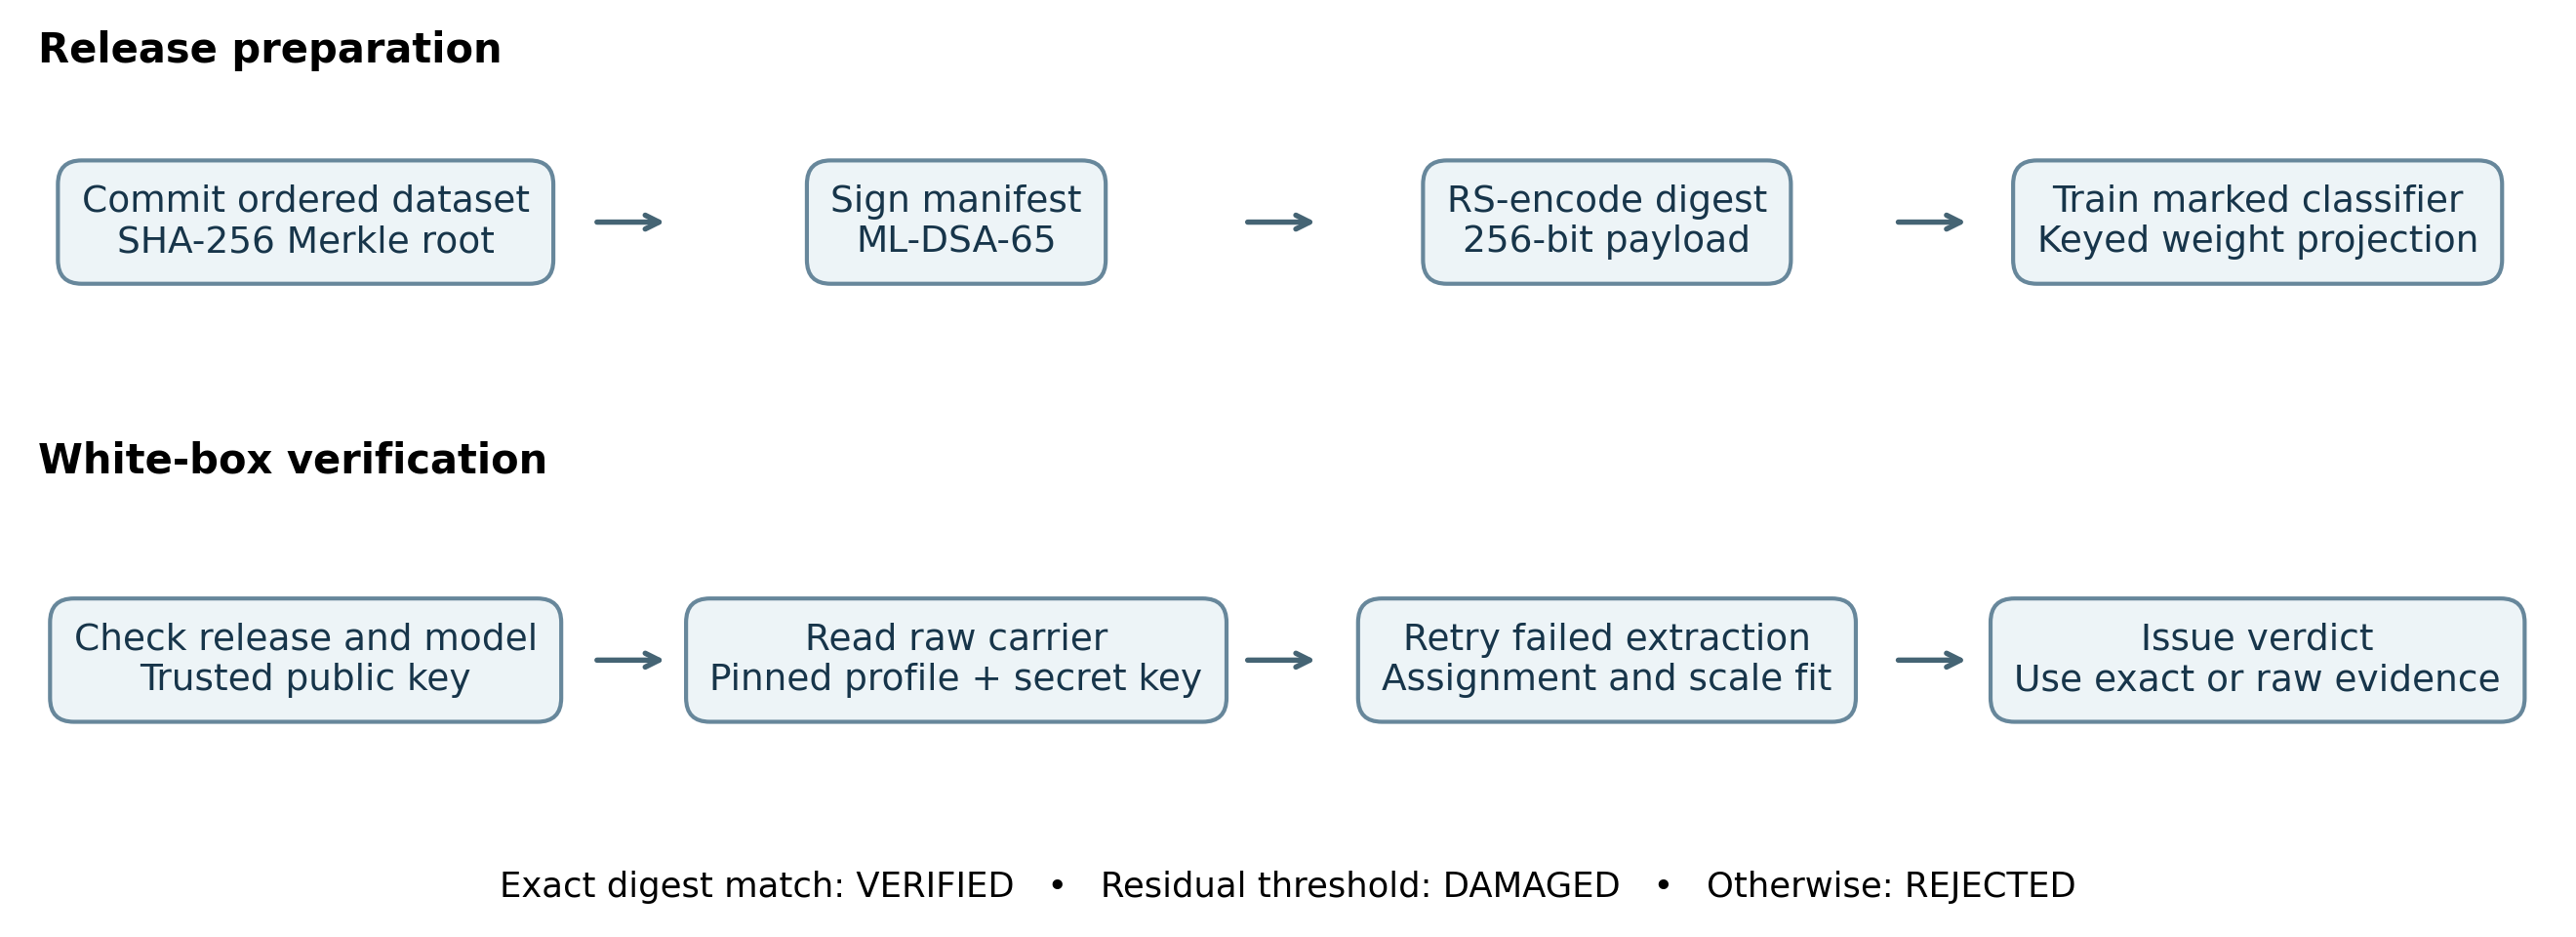
\includegraphics[width=0.96\textwidth]{figures/00_architecture.png}
\caption{End-to-end post-quantum provenance protocol. Top: the developer commits to the ordered CIFAR-10 training set via a SHA-256 Merkle tree, signs a canonical manifest with ML-DSA-65, and embeds its Reed--Solomon-encoded 256-bit digest into \textsc{SmallCNN} via a keyed projection. Bottom: the white-box auditor verifies the signature and tensor integrity, decodes the watermark with soft erasures, applies Cover-bounded alignment when needed, and issues \textsc{Verified}, \textsc{Damaged}, or \textsc{Rejected}.}\label{fig:arch}
\end{figure*}

\subsection{Actors, Threat Model, and Scope}
Our protocol (Fig.~\ref{fig:arch}) involves two parties: a \textbf{Developer}, who commits to a training dataset, signs a release manifest, and trains a watermarked classifier; and a \textbf{Trusted Auditor}, who holds white-box access to a suspect model checkpoint alongside the developer's public key, signed manifest, and secret watermark key~\cite{projectResults}. We model three adversaries:
\begin{enumerate}
  \item \textbf{Remover:} Possesses the model weights and applies post-training modifications---Gaussian noise, magnitude pruning, quantization, fine-tuning, function-preserving channel permutation or scaling, or same-layer watermark overwriting---to erase provenance while keeping classification accuracy within 5 percentage points of the clean watermarked model.
  \item \textbf{Forger:} Attempts to pass off an unmarked or third-party model as the developer's release by altering manifest fields, forging signatures, or exploiting weak verification rules (such as checking only a short prefix of the payload).
  \item \textbf{Poisoner:} Modifies, re-labels, or reorders training samples after the dataset commitment has been signed.
\end{enumerate}

To keep all claims defensible, we state four explicit boundaries: (i)~verification is white-box and assumes a trusted auditor who protects the secret watermark key; (ii)~the dataset Merkle root proves \emph{which} dataset was committed at signing time, not that samples were clean beforehand or that the weights were trained exclusively on those samples; (iii)~model distillation (training a new model from API outputs) is out of scope; and (iv)~manifest timestamps are self-declared, so ownership priority disputes require an external timestamping authority (e.g., RFC~3161) or transparency log.

\subsection{Dataset Commitment and ML-DSA-65 Manifest Signing}
To bind all 50,000 ordered CIFAR-10 training images~\cite{cifar10} into a compact commitment, the developer constructs a domain-separated SHA-256 Merkle tree~\cite{merkle1987digital}. Each leaf hashes a domain tag, sample index, label, and raw uint8 pixel bytes:
\begin{equation}
  h_i = \mathrm{SHA256}\bigl(\texttt{0x00} \parallel \mathrm{u64be}(i) \parallel \mathrm{u16be}(y_i) \parallel \mathbf{x}_i\bigr),
\end{equation}
while internal nodes hash $\texttt{0x01} \parallel h_{\mathrm{left}} \parallel h_{\mathrm{right}}$ (promoting odd nodes unchanged). Domain separation prevents second-preimage confusion between leaves and internal nodes, and embedding the index $i$ prevents silent sample reordering.

The resulting 32-byte root is placed in a canonical JSON manifest (sorted keys, no extraneous whitespace) containing the developer identifier, public-key identifier ($\mathrm{SHA256}(pk)_{[0:16]}$), architecture (\textsc{SmallCNN}, width 32, 160,234 parameters), watermark payload bit length (256), and UTC timestamp. The developer signs the exact canonical manifest bytes $M$ using \textbf{ML-DSA-65} (NIST FIPS~204~\cite{nist204}), producing a 3,309-byte signature verifiable under a 1,952-byte public key. Because embedding 26,472 signature bits directly inside a 160k-parameter network is impractical, the signed manifest ships beside the release while the watermark payload is defined as the full 256-bit digest
\begin{equation}
  p = \mathrm{SHA256}(M) \in \{0,1\}^{256}.
\end{equation}
Excluding $p$ from $M$ avoids circularity, while ensuring that altering any manifest field flips roughly half of the embedded payload bits.

\subsection{Error-Corrected Projection Watermarking}
Before training, the 32-byte payload $p$ is encoded with a systematic Reed--Solomon (RS) code over $\mathrm{GF}(256)$~\cite{reed1960polynomial}: \textbf{RS32} appends 32 parity bytes to yield $n=512$ binary codeword bits (correcting $e$ byte errors and $f$ erasures whenever $2e+f \le 32$), whereas \textbf{RS16} appends 16 parity bytes to yield $n=384$ bits ($2e+f \le 16$).

Following Uchida \emph{et al.}~\cite{uchida2017embedding}, we select the final convolutional layer (\texttt{features.6.0.weight}, shape $128 \times 64 \times 3 \times 3$) and average across its 128 output filters to obtain a 576-element carrier vector $v \in \mathbb{R}^{576}$ ($C=64$ input channels $\times K=9$ spatial taps). Output-channel averaging makes the carrier intrinsically invariant to permuting the carrier's output filters. A 32-byte secret watermark key is expanded deterministically with SHAKE-256 into a projection matrix $X \in \{-1,+1\}^{n \times 576}$, producing raw projection logits $z = Xv \in \mathbb{R}^n$.

Let $s_i = 2b_i - 1 \in \{-1,+1\}$ denote the signed target for codeword bit $b_i \in \{0,1\}$. The model is trained jointly with classification cross-entropy $\mathcal{L}_{\mathrm{CE}}$ and a weighted watermark objective $\mathcal{L}_{\mathrm{total}} = \mathcal{L}_{\mathrm{CE}} + \lambda \mathcal{L}_{\mathrm{wm}}$ comparing two formulations:
\begin{align}
  \mathcal{L}_{\mathrm{BCE}} &= \frac{1}{n}\sum_{i=1}^{n} \log\!\bigl(1 + \exp(-s_i z_i)\bigr), \label{eq:bce}\\
  \mathcal{L}_{\mathrm{hinge}} &= \frac{1}{n}\sum_{i=1}^{n} \max\bigl(0,\, m - s_i z_i\bigr). \label{eq:hinge}
\end{align}
Both penalize sign errors, but their gradients diverge sharply once a bit is correctly embedded. Because $\mathcal{L}_{\mathrm{BCE}}$ never vanishes, SGD continues enlarging the shared mean filter $v$ until weight decay counterbalances it, crowding out per-filter discriminative features. In contrast, $\mathcal{L}_{\mathrm{hinge}}$ contributes zero loss and zero gradient once $s_i z_i \ge m$, preserving classification capacity at the expense of leaving individual projection scores close to the boundary $m$.

\subsection{White-Box Verification, Obfuscation Recovery, and Verdicts}
Given a suspect checkpoint, release manifest, trusted public key, and watermark key, the auditor runs a strict staged pipeline~\cite{projectResults}:
\begin{enumerate}
  \item \textbf{Cryptographic and structural checks:} Verify the ML-DSA-65 signature on $M$, verify key-ID consistency, load checkpoint tensors safely without Python unpickling (rejecting crafted pickle payloads), check exact parameter count at signed width 32, reject any \texttt{NaN}/\texttt{Inf} weights, and enforce full 256-bit payload verification (preventing short-prefix forgery).
  \item \textbf{Soft-erasure RS decoding:} Compute $z = Xv$, map signs $\mathbb{I}[z_i > 0]$ to received bytes, and assign each byte a confidence equal to its smallest bit magnitude $\min_{j \in \text{byte}} |z_j|$. Plain RS decoding is tried first, followed by erasing the $2, 4, \dots, p/2$ least-confident bytes. Capping erasures at $p/2$ retains $p/2$ parity bytes for error detection; without this cap, pure Gaussian noise ``decoded'' 1,000/1,000 times, whereas with the cap 0/1,000 noise inputs decode. Exact recovery requires the decoded 256 bits to match $\mathrm{SHA256}(M)$ identically, yielding \textsc{Verified}.
  \item \textbf{Cover-bounded structural-obfuscation recovery:} Permuting or positively rescaling the $C=64$ input channels feeding the carrier conv (compensated in the preceding BatchNorm/conv block, as in~\cite{yan2023rethinking}) preserves the classifier's exact function while scrambling $v$. Viewing $v$ as $C$ blocks $v_c \in \mathbb{R}^K$ and writing $A = (X^\top s) \in \mathbb{R}^{C \times K}$, the alignment score of channel permutation $\pi$ decomposes linearly across slots:
  \begin{equation}
    \sum_{j=1}^{n} s_j (X v_\pi)_j = \sum_{c=1}^{C} A_c \cdot v_{\pi(c)},
  \end{equation}
  which the verifier solves exactly via the Hungarian algorithm~\cite{kuhn1955hungarian}. To reverse positive per-channel scaling $v_c \mapsto v_c / s_c$, the verifier solves a 65-variable, $n$-constraint HiGHS linear program maximizing worst-case margin $t$ over positive scales $a_1, \dots, a_C \ge 10^{-3}$ subject to $\sum_{c=1}^{C} a_c = C$ and $\sum_{c=1}^{C} a_c s_j (X_{j,c} \cdot v_c) \ge t$ for all $j$, plus a combined pass applying Hungarian matching to $\ell_2$-normalized blocks followed by scale LP. Each candidate is accepted \emph{only} if RS decoding yields an exact 256-bit match with $\mathrm{SHA256}(M)$. Crucially, alignment is permitted only when Cover's function-counting bound~\cite{cover1965geometrical},
  \begin{equation}
    \log_2 P_{\mathrm{cover}}(n, C) = \log_2\!\left(2^{1-n}\sum_{k=0}^{C-1}\binom{n-1}{k}\right) \le -64,
  \end{equation}
  proves that $C$ linear scale degrees of freedom cannot spuriously realize an arbitrary $n$-bit sign pattern. For $C=64$, this bound is $2^{-239.7}$ for RS32 ($n=512$) and $2^{-139.9}$ for RS16 ($n=384$), whereas a legacy 32-bit code over $C=16$ channels yields $2^{-1.0}$ and is automatically refused.
  \item \textbf{Residual-evidence verdict (\textsc{Damaged}):} If exact decoding fails after signature and structural checks pass (e.g., following a watermark overwrite), the auditor counts raw sign agreements $k = \sum_{j=1}^{n}\mathbb{I}[s_j z_j > 0]$ in the checkpoint's \emph{original, unaligned} channel order. Under an unmarked null model, $k \sim \mathrm{Binomial}(n, 1/2)$. For RS32 ($n=512$), observing $k \ge 358$ has exact upper-tail probability $2^{-64.2} < 2^{-64}$ and yields \textsc{Damaged}---statistical evidence that the model derives from the signed release despite exact-payload destruction. Insufficient evidence or any failed cryptographic/structural check yields \textsc{Rejected}.
\end{enumerate}

\section{Experimental Evaluation}
\label{sec:evaluation}

\subsection{Experimental Setup}
We use CIFAR-10's 50,000 training and 10,000 test images~\cite{cifar10} and \textsc{SmallCNN} (width 32, five $3\times3$ Conv--BatchNorm--ReLU blocks, three max-pooling stages, dropout 0.3, and a ten-class head). Training uses random crop (padding 4), horizontal flip, SGD with Nesterov momentum 0.9 and weight decay $5\times10^{-4}$, batch size 128, and a 30-epoch cosine schedule starting at 0.05. The reported Colab training setup uses a Tesla T4. The main watermark runs use the final convolution in mean mode, $\lambda=20$, a full 256-bit payload, and $m=1.5$ for hinge.

Clean accuracy uses five trained checkpoints each for the unmarked baseline, BCE/RS32, and hinge/RS32 (seeds 0--4), and three for BCE/RS16 (seeds 0--2). Robustness uses three parent checkpoints per watermark design (seeds 0--2). Each parent supplies 84 evaluations across 47 modification configurations and one clean control. Eighteen configurations use three draws and thirty use one, including the control. The 252 evaluations per design reuse the same three trained models, release, watermark key, and test set. Stochastic attack repeats do not add independent training runs.

The suite covers Gaussian noise relative to tensor spread (multipliers 0.01--0.5 broadly and 0.1--1.0 on the carrier), global and per-layer magnitude pruning (10--95\% and 30--90\%, respectively), pruning followed by three fine-tuning epochs, FP16 and per-tensor/per-channel quantization, fine-tuning (up to ten epochs), channel permutation and rescaling, and same-layer watermark overwriting. The 128- and 512-bit overwrites use ten epochs on a 20\% training subset at $\lambda=20$ and learning rate 0.01~\cite{projectResults}. We report the verifier verdict and test accuracy separately. A \emph{successful removal} requires \textsc{Rejected} and a test accuracy drop of at most five percentage points from that parent model's clean accuracy. This is a relative budget and does not specify an absolute accuracy requirement.

\subsection{Clean Accuracy and Carrier Measurements}
Table~\ref{tab:clean-acc} and Fig.~\ref{fig:accuracy} report the clean results. The saved training summaries report zero decoded payload errors for the 13 marked checkpoints in the table. Over five paired seeds, BCE/RS32 averaged 82.37\% ($-2.23$ points relative to baseline, paired SD 2.18 points), and hinge/RS32 averaged 84.10\% ($-0.50$ points, paired SD 1.79). The hinge-minus-BCE difference was positive in all five pairs (range 0.92--2.40 points, mean 1.73). For seeds 0--2, BCE/RS16 averaged 82.26\% ($-2.81$ points relative to the same-seed baselines) and BCE/RS32 averaged 81.98\% ($-3.10$ points). RS16 embeds 128 fewer coded bits for the same payload.

\begin{table}[!t]
\centering
\caption{Paired Clean CIFAR-10 Test Accuracy (\%)}
\label{tab:clean-acc}
\footnotesize
\begin{tabular}{@{}lrrrr@{}}
\toprule
Seed & Baseline & BCE/RS16 & BCE/RS32 & Hinge/RS32 \\
\midrule
0 & 86.12 & 82.09 & 83.08 & 84.79 \\
1 & 85.32 & 80.75 & 80.33 & 82.73 \\
2 & 83.78 & 83.95 & 82.52 & 84.69 \\
3 & 81.98 & ---   & 82.84 & 83.76 \\
4 & 85.78 & ---   & 83.07 & 84.53 \\
\midrule
Mean & 84.60 & 82.26 & 82.37 & 84.10 \\
Paired $\Delta$ (pt) & --- & $-2.81$ & $-2.23$ & $-0.50$ \\
\bottomrule
\end{tabular}
\end{table}

\begin{figure}[!tb]
\centering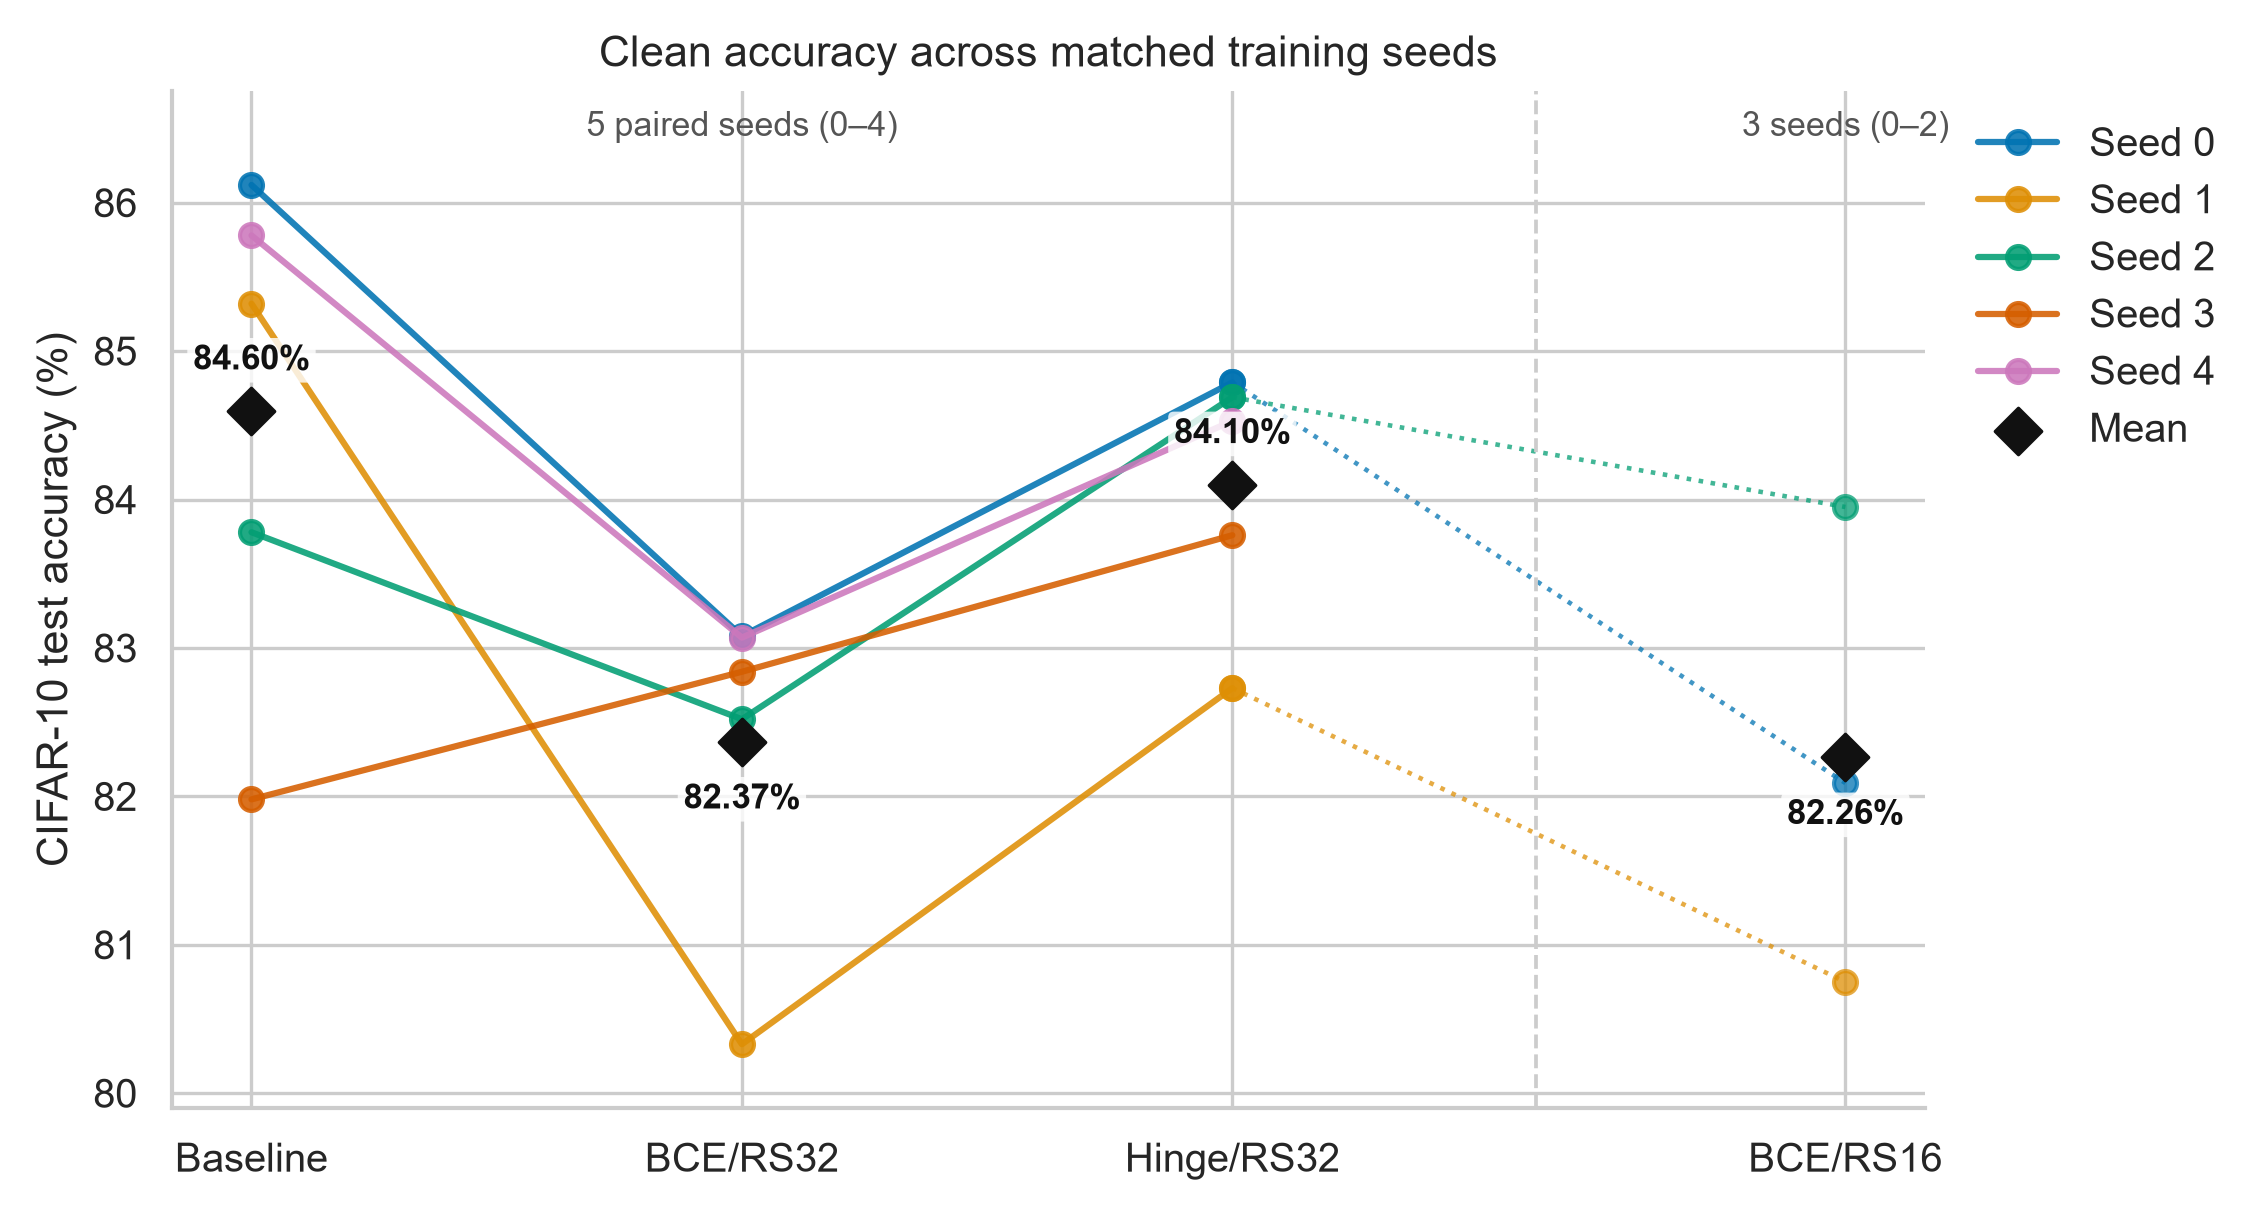
\includegraphics[width=\columnwidth]{figures/01_paired_accuracy.png}
\caption{Clean CIFAR-10 accuracy across paired training seeds. Hinge/RS32 uses $m=1.5$. BCE/RS16 is available for seeds 0--2.}\label{fig:accuracy}
\end{figure}

Table~\ref{tab:weight-split} and Fig.~\ref{fig:mechanism} describe the carrier rather than a causal mechanism. For $W$ with 128 flattened filters, shared energy is $128\|v\|_2^2/\|W\|_F^2$ and the residual norm is the mean across filters of $\|W_j-v\|_2$. Across seeds 0--2 the shared norm was about 5.05 for BCE/RS32 and 2.39 for hinge/RS32, with shared energy about 97\% and 88--89\%, respectively. The minimum absolute logit across the saved clean runs for each main design was 2.24 for BCE/RS32, 2.70 for BCE/RS16, and 1.50 for hinge/RS32. These measurements document differences accompanying the loss choice. They do not isolate the role of the shared norm or margin in either accuracy or overwrite resistance.

\begin{figure*}[!t]
\centering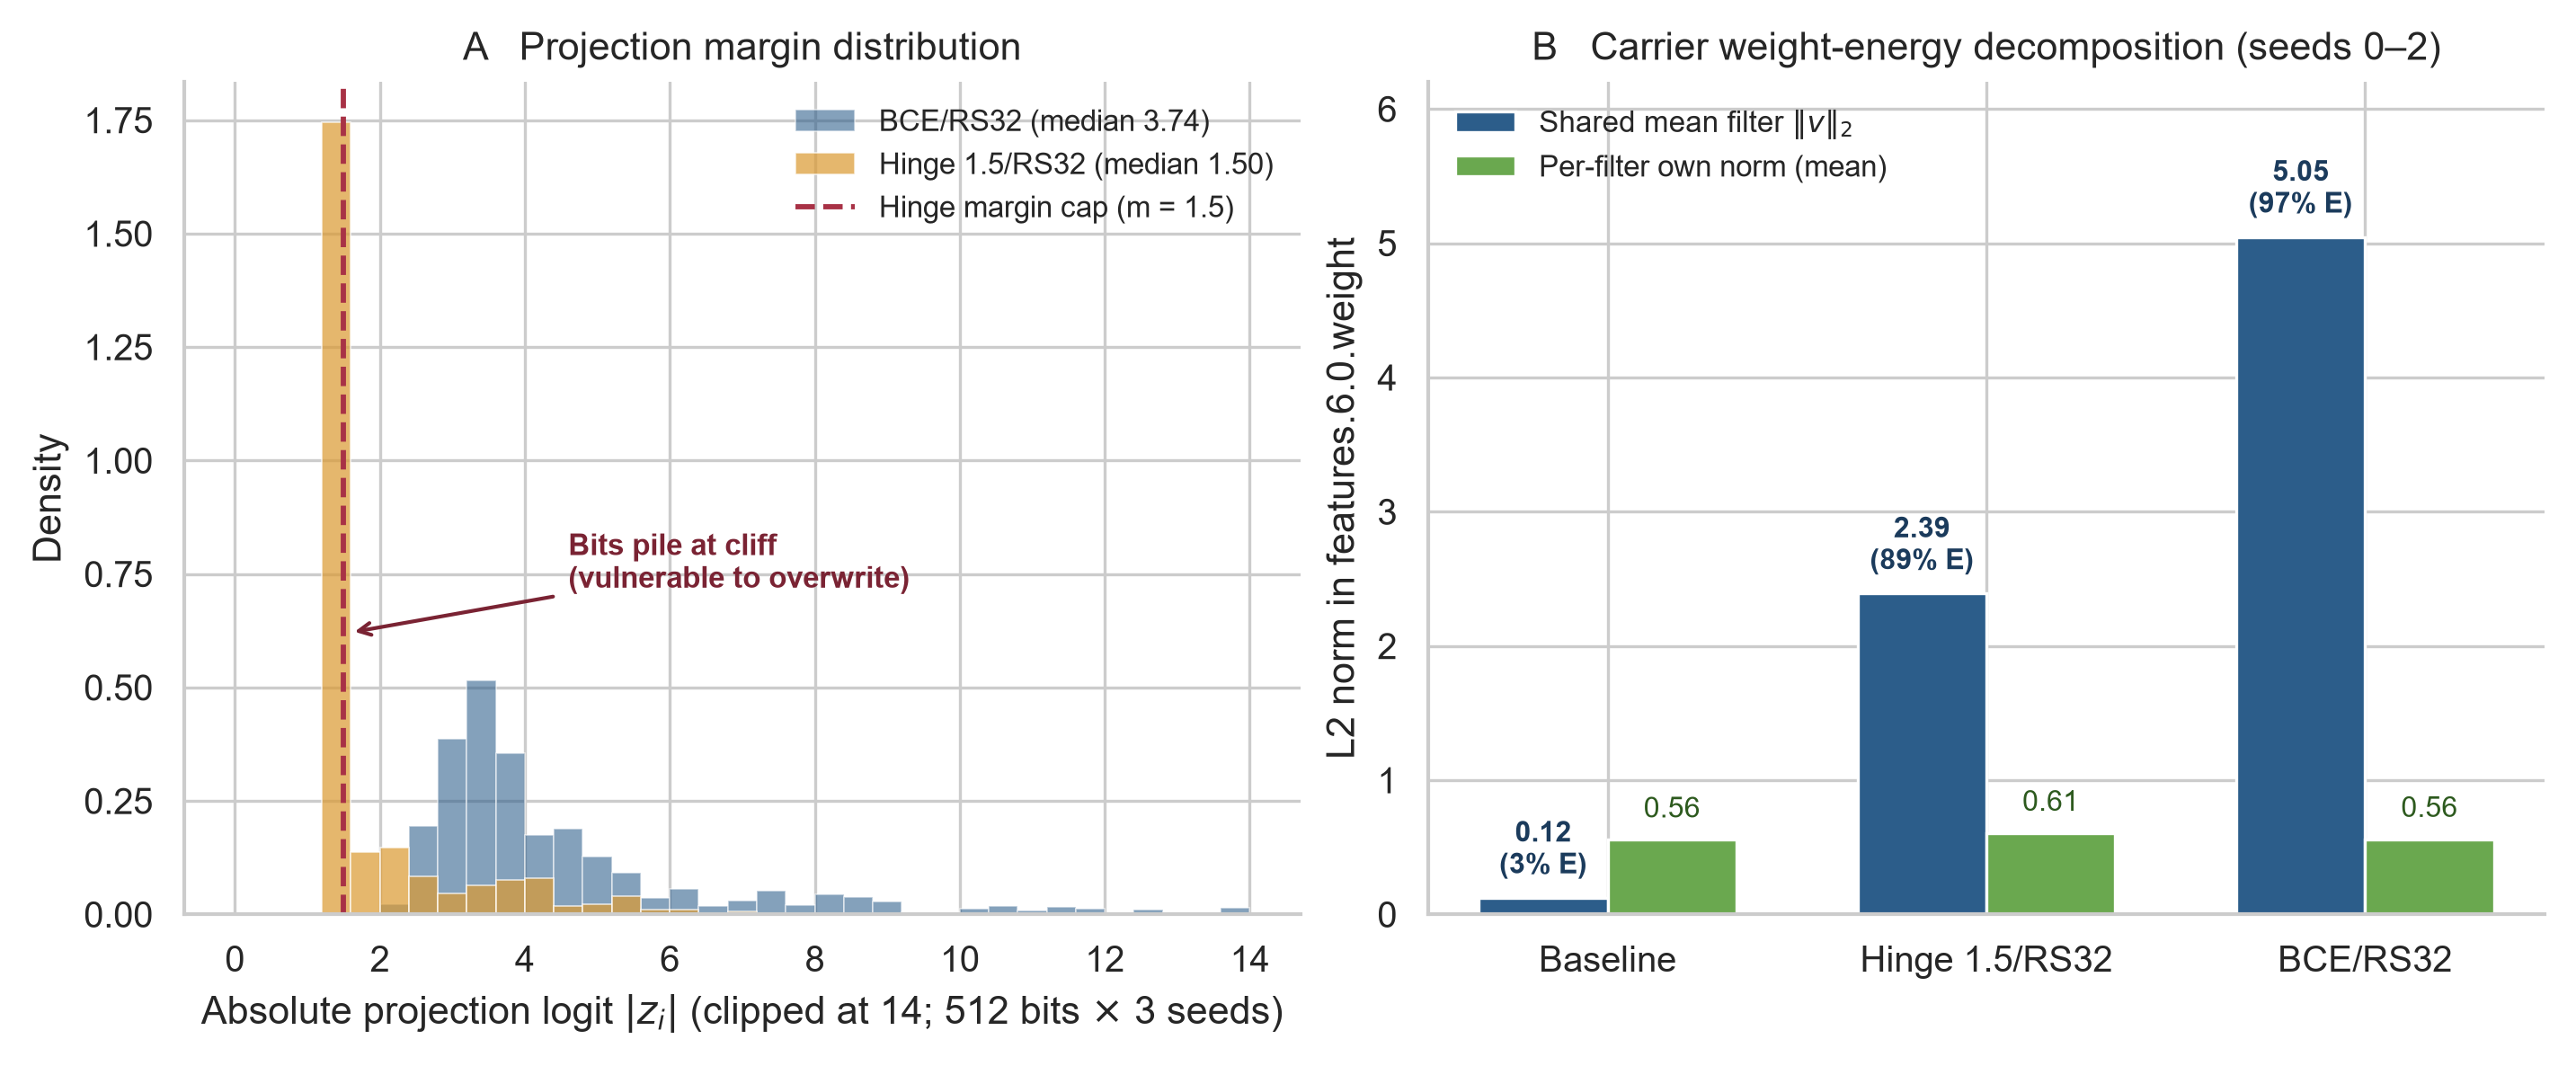
\includegraphics[width=0.90\textwidth]{figures/06_mechanism_bce_vs_hinge.png}
\caption{Carrier decomposition recomputed from the saved checkpoints for seeds 0--2. Each point is a trained model. Panels show the shared mean-filter norm and the fraction of layer energy in that mean.}\label{fig:mechanism}
\end{figure*}

\begin{table}[!t]
\centering
\caption{Carrier Decomposition, Seeds 0--2}
\label{tab:weight-split}
\footnotesize
\setlength{\tabcolsep}{3pt}
\begin{tabular}{@{}lrrrr@{}}
\toprule
Design & Shared & Residual & Ratio & Energy \\
\midrule
Baseline & 0.11--0.13 & 0.47--0.60 & 0.2 & 2--3\% \\
Hinge 1.5/RS32 & 2.39 & 0.57--0.67 & 3.6--4.2 & 88--89\% \\
Hinge 2.5 (seed 0) & 3.98 & 0.56 & 7.1 & 96\% \\
BCE/RS32 & 5.05 & 0.51--0.62 & 8.2--10.0 & 97\% \\
\bottomrule
\end{tabular}
\end{table}

At seed 0, the BCE/RS32 strength sweep used $\lambda=1,5,20$. The corresponding minimum absolute logits were 0.02, 1.21 and 2.25, with clean accuracies of 84.67\%, 83.19\% and 83.08\% (Fig.~\ref{fig:strength}). These are three recorded runs at one seed.

\begin{figure}[!tb]
\centering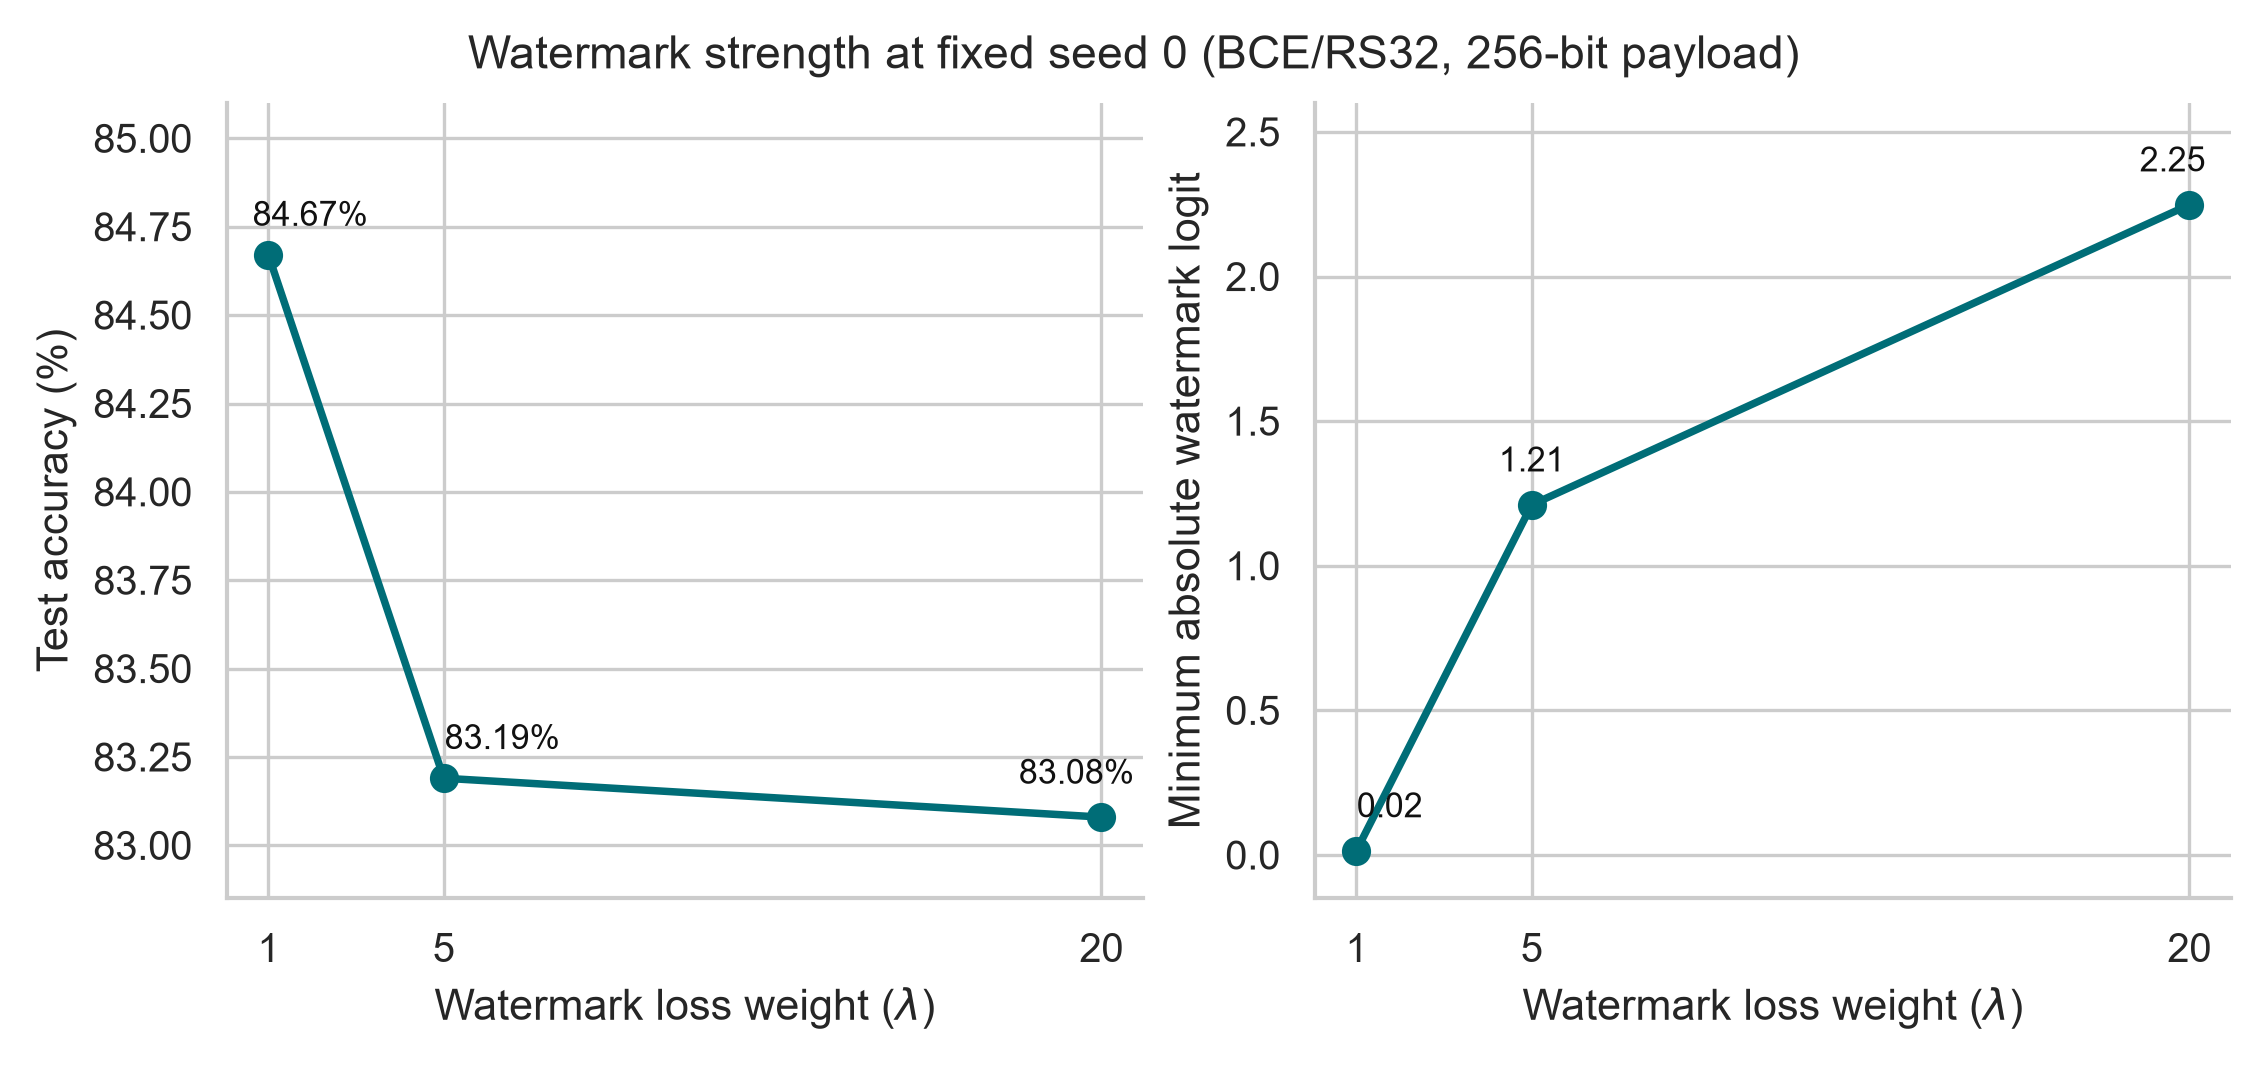
\includegraphics[width=\columnwidth]{figures/03_strength_seed0.png}
\caption{Strength sweep at fixed seed 0, carrier layer, BCE loss and 256-bit payload with RS32.}\label{fig:strength}
\end{figure}

\subsection{Verification, Utility, and Overwrite}
Table~\ref{tab:robustness} and Fig.~\ref{fig:robust} summarize saved verdicts. Exact recovery occurred even on checkpoints with large accuracy losses. For example, all three BCE/RS32 checkpoints verified after 70\% global pruning (mean accuracy 16.48\%) and after 3-bit per-tensor quantization (24.41\%). At 3 bits, the raw sign-change rate relative to the clean checkpoint averaged 1.11\%, hard RS decoding corrected 5.33 bytes on average with zero erasures on all three evaluations, and accuracy fell by 57.57 points on average (Fig.~\ref{fig:ecc}). At 2 bits, the three BCE/RS32 evaluations averaged 9.53\% accuracy. The rejected checkpoint scored 8.58\%.

Across the three designs, all 108 evaluations of output, input, or all-layer permutations and the combined permutation with $\times10$ input scaling verified. All 81 evaluations of input scaling alone also verified. Recorded test accuracy was unchanged in these 189 cases. All 81 separate output-side rescaling evaluations verified, with recorded accuracy changes of up to 0.07 points in absolute value. Figure~\ref{fig:align}A displays recorded structural results from the verifier with retries available. The figure does not estimate how many would verify with retries disabled.

\begin{table}[!t]
\centering
\caption{Saved Verdicts Across 252 Evaluations per Design}
\label{tab:robustness}
\footnotesize
\setlength{\tabcolsep}{3pt}
\begin{tabular}{@{}lrrrr@{}}
\toprule
Design & Verified & Damaged & Rejected & Removals \\
\midrule
BCE/RS32 & 231 & 20 & 1 & 0 \\
BCE/RS16 & 240 & 12 & 0 & 0 \\
Hinge/RS32 & 233 & 13 & 6 & 3 \\
\bottomrule
\end{tabular}
\end{table}

\begin{figure*}[!t]
\centering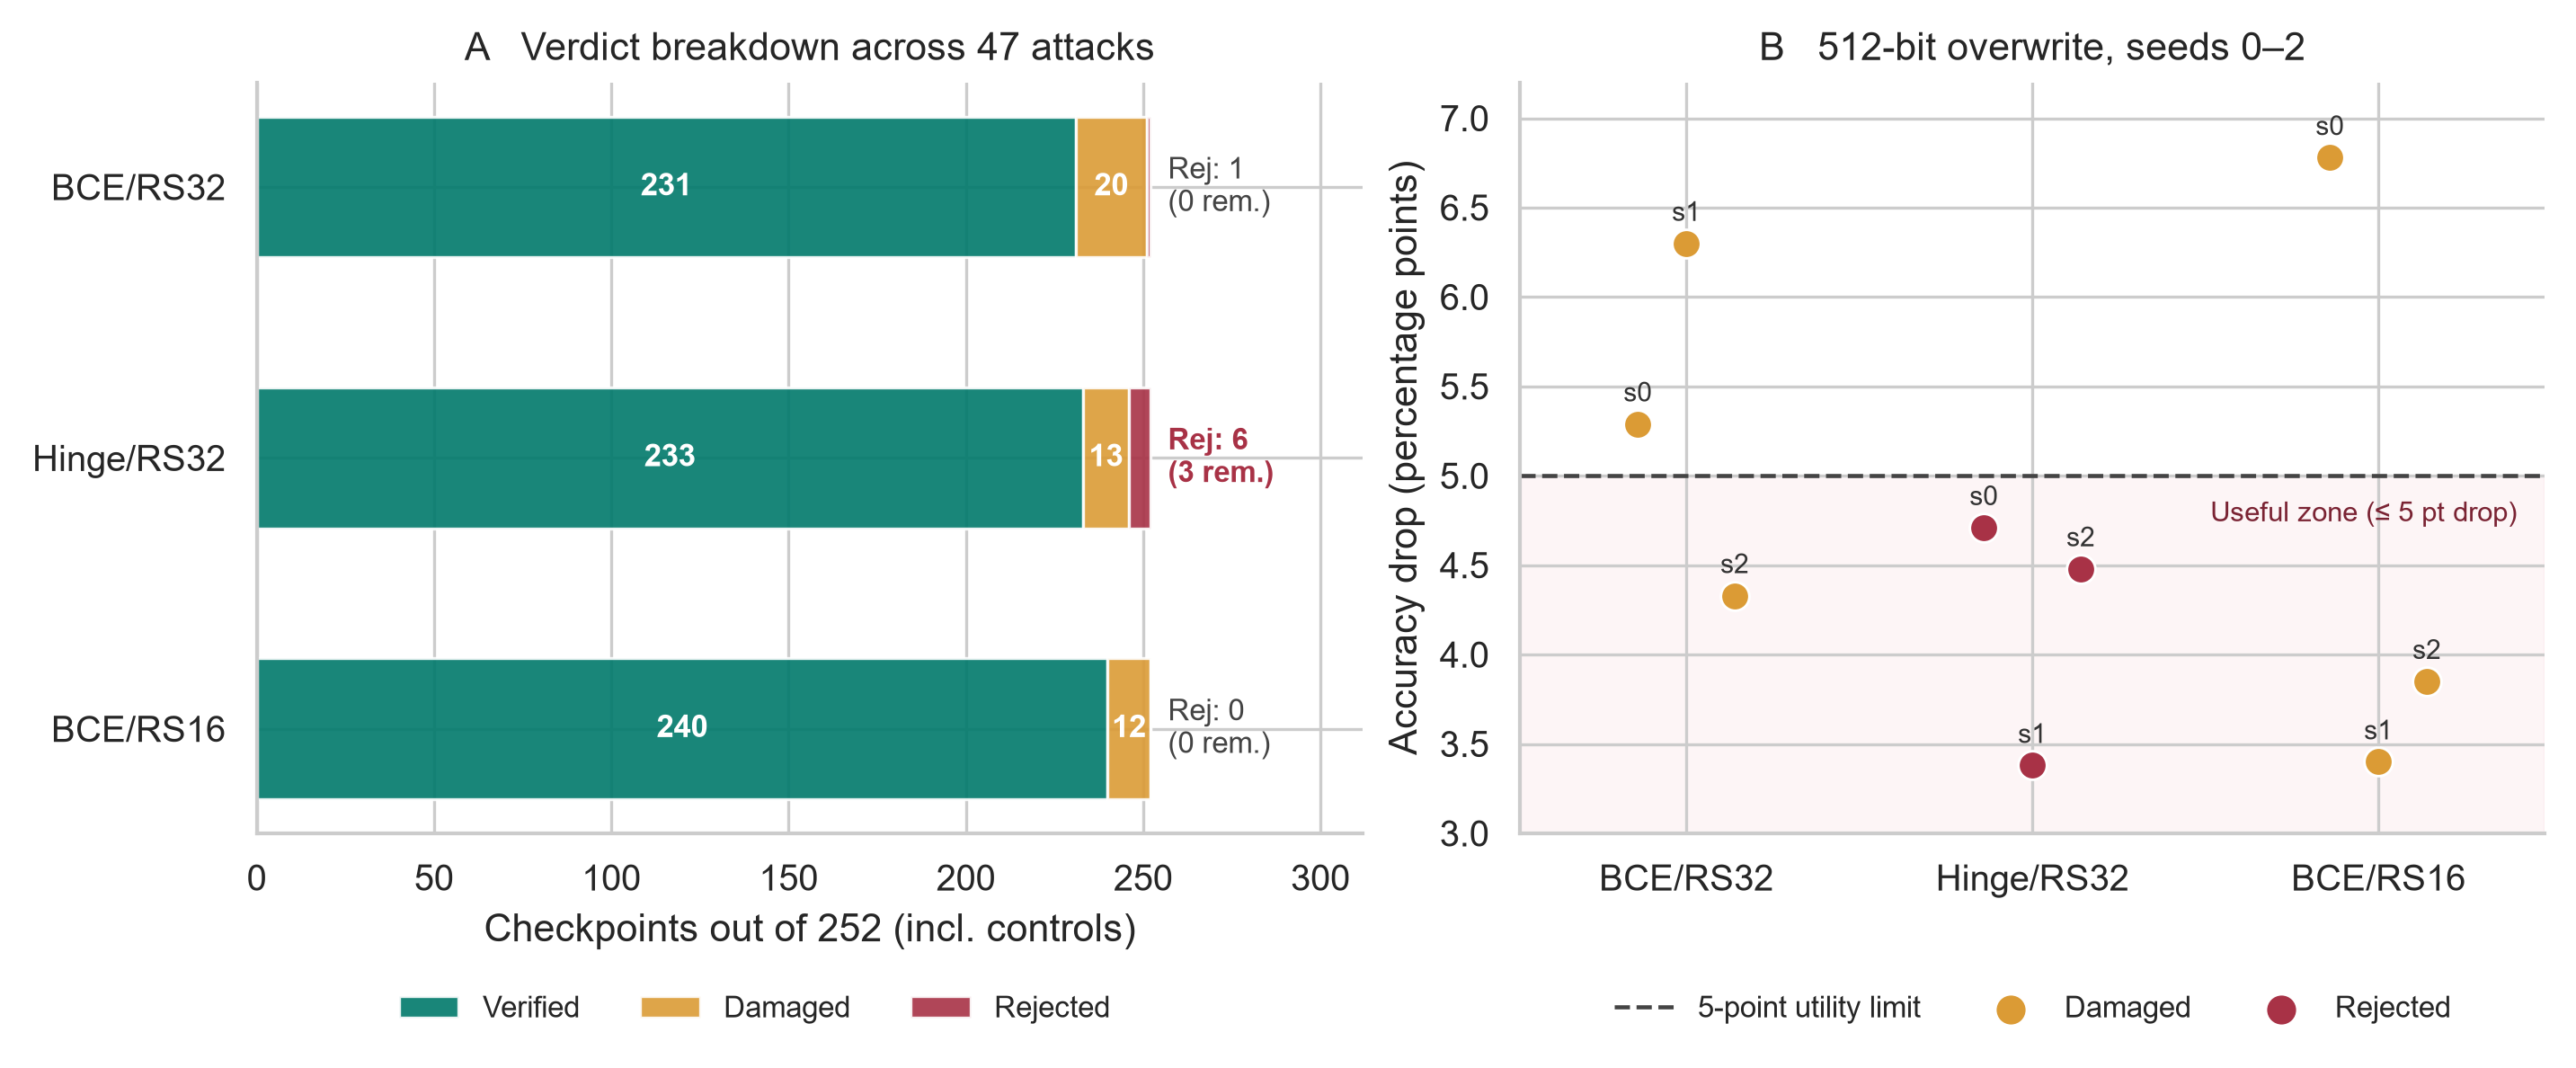
\includegraphics[width=0.90\textwidth]{figures/02_robustness.png}
\caption{Left: verdict counts, including three clean controls per design. Right: per-seed accuracy drop and verdict under a 512-bit same-layer overwrite. The three hinge rejections meet the five-point budget. All six BCE evaluations yield \textsc{Damaged}, including three within that budget.}\label{fig:robust}
\end{figure*}

Applying the utility filter row by row, the numbers of \textsc{Verified} evaluations within five points were 179, 181 and 184 for BCE/RS32, BCE/RS16 and hinge/RS32, respectively (176, 178 and 181 excluding their clean controls). In the 512-bit overwrite setting, hinge was rejected at drops of 4.71, 3.38 and 4.48 points, with 32.4--36.3\% of raw signs changed relative to the clean checkpoint. The other three hinge rejections were at 2-bit quantization (mean accuracy 9.90\%). The 512-bit BCE results were all \textsc{Damaged}. Their raw sign-change ranges were 20.3--25.0\% for RS32 and 15.9--24.2\% for RS16. One RS32 and two RS16 evaluations met the accuracy budget. Under the 128-bit overwrite, BCE/RS16 verified exactly in all three trials. There were zero successful removals for either BCE design in the recorded suite. Although hinge returned more exact matches than BCE/RS32 overall, the utility-filtered rejections expose an overwrite tradeoff.

\begin{figure}[!tb]
\centering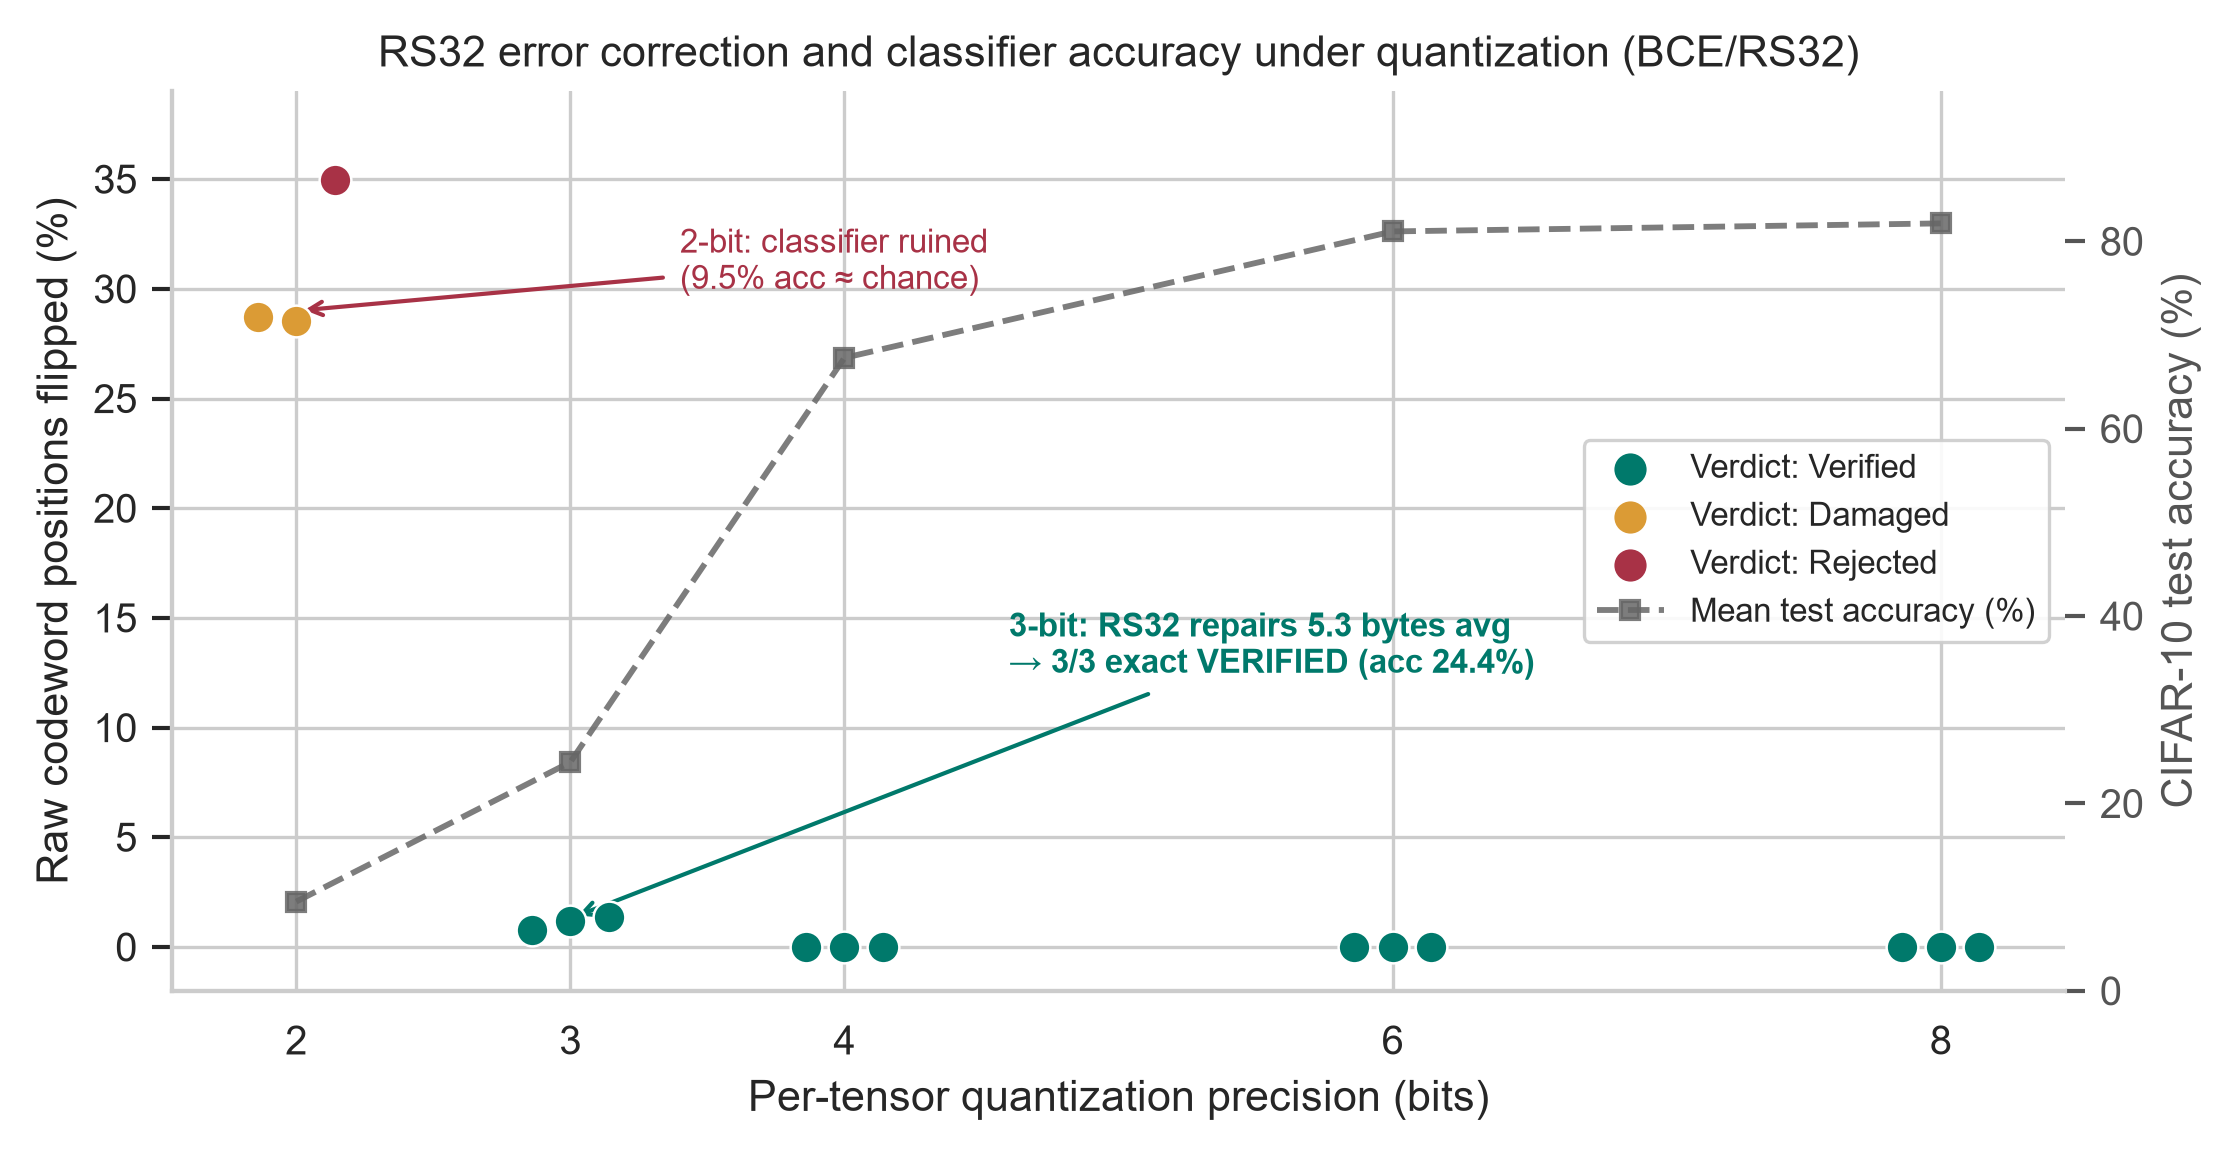
\includegraphics[width=\columnwidth]{figures/05_ecc_quantization.png}
\caption{BCE/RS32 per-tensor quantization across three seeds. The 3-bit checkpoints verified with byte corrections and zero erasures. At 2 bits, the mean accuracy was 9.53\% and the verdicts were two \textsc{Damaged} and one \textsc{Rejected}.}\label{fig:ecc}
\end{figure}

\subsection{RS32 Controls and Auxiliary Baseline}
We observed zero exact or residual detections in 724 RS32 extraction controls and zero in 54 attacked unmarked baseline evaluations (Table~\ref{tab:fp}). The extraction study includes 600 wrong-key trials on three marked checkpoints, and reuses checkpoints in several other groups. Its maximum recorded raw agreement was 305 of 512 (Fig.~\ref{fig:null}). The 54 attacked baselines are a separate cohort with saved verifier verdicts. These observations are specific to the sampled cases. They do not estimate the false-accept probability for an adaptive adversary or for RS16.

\begin{table}[!t]
\centering
\caption{RS32 Negative Controls}
\label{tab:fp}
\footnotesize
\setlength{\tabcolsep}{3pt}
\begin{tabular}{@{}lrrrr@{}}
\toprule
Cohort & Cases & False V/D & Mean & Max. \\
\midrule
Wrong watermark key & 600 & 0/0 & 256.2 & 305 \\
Unmarked baseline & 3 & 0/0 & 253.3 & 256 \\
Scrambled baseline & 15 & 0/0 & 258.5 & 278 \\
Third-party model & 1 & 0/0 & 264.0 & 264 \\
Scrambled third-party & 5 & 0/0 & 259.2 & 265 \\
Random initialization & 100 & 0/0 & 256.1 & 289 \\
Attacked baseline & 54 & 0/0 & --- & --- \\
\midrule
Total & 778 & 0/0 & --- & --- \\
\bottomrule
\end{tabular}
\end{table}

\begin{figure}[!tb]
\centering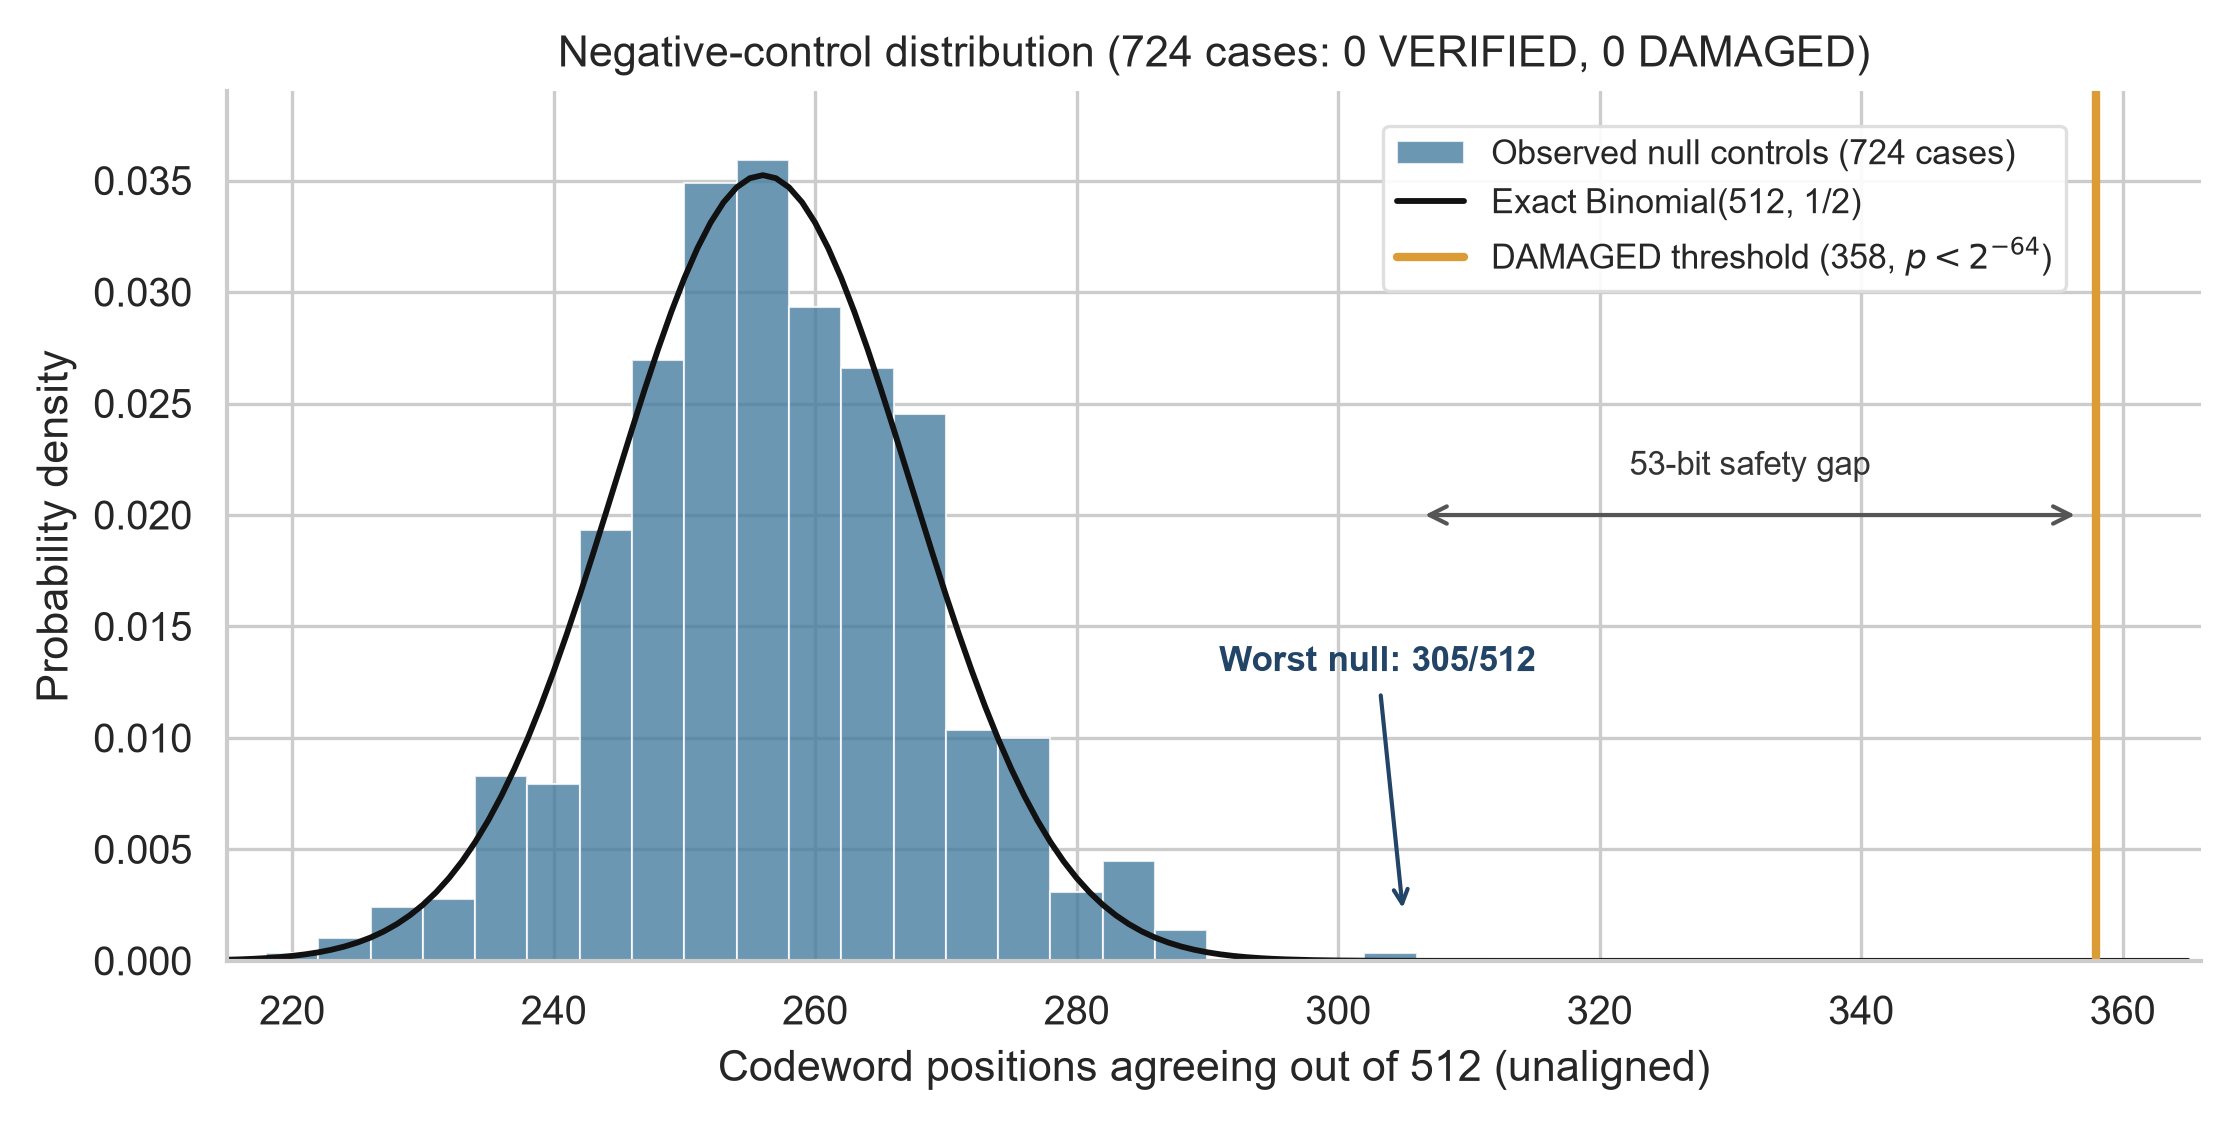
\includegraphics[width=\columnwidth]{figures/04_false_positive_controls.png}
\caption{Observed raw agreement across the 724 RS32 extraction controls. The vertical line marks the decision threshold at 358 of 512. The separate attacked-baseline cohort is excluded.}\label{fig:null}
\end{figure}

An exploratory comparison assigns each RS32 bit to the sign of one keyed weight after training (Fig.~\ref{fig:align}B). The naive mark reduced clean accuracy by 0.09 points on average across two seeds. It was removed within budget in six configurations. Averaging equally over the 36 common non-control weight-attack settings, the exact verification rates were 26\% for the naive method and 86\% for the BCE/RS32 projection pipeline. The combined exact-or-residual rates were 61\% and 99\%. The naive extractor has no alignment retry. It uses two seeds and one draw per stochastic setting, compared with three seeds and three draws for projection. These are descriptive pipeline comparisons.

\begin{figure*}[!t]
\centering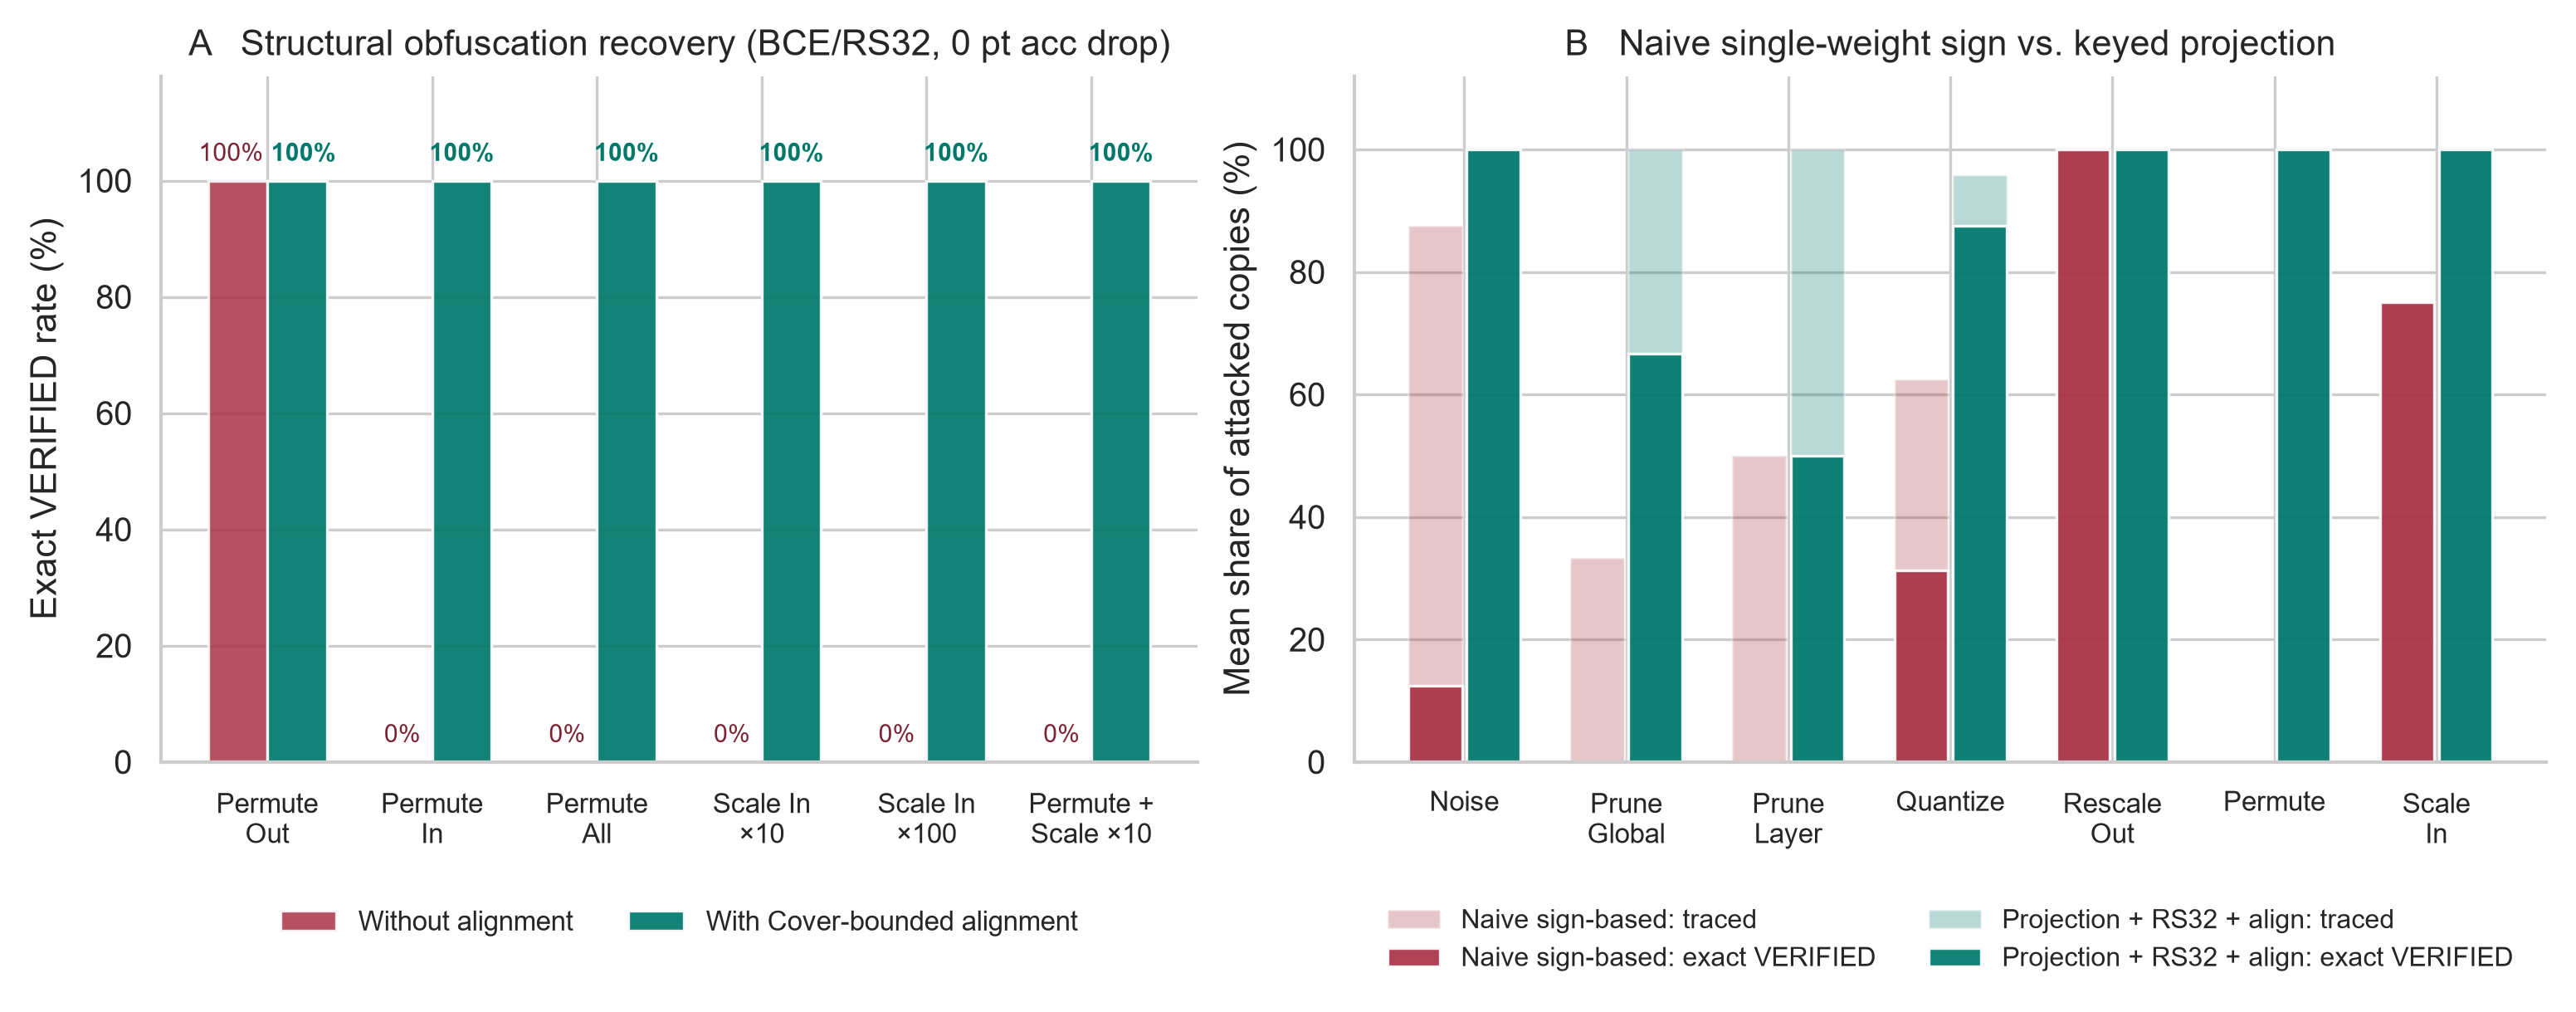
\includegraphics[width=0.96\textwidth]{figures/07_alignment_and_attacks.png}
\caption{(A) Mean raw sign changes relative to the clean checkpoints, with exact verdict counts from the verifier with retries available. Each configuration has nine recorded evaluations per design. (B) Recorded exact and exact-or-residual rates for the naive and projection pipelines, averaged equally across common configurations within each family. The baseline evaluation uses different seed and repeat counts.}\label{fig:align}
\end{figure*}

\section{Discussion and Conclusion}
\label{sec:conclusion}
In this \textsc{SmallCNN}/CIFAR-10 evaluation, changing from BCE to hinge with RS32 improved clean accuracy across the five paired runs. In the specified 512-bit overwrite, all three hinge checkpoints were rejected within the stated utility budget, while both BCE designs retained residual agreement in all tested repeats. The carrier measurements accompany these outcomes. Matched-margin and strength controls would be needed to assess whether either quantity accounts for the observed difference.

The benchmark uses one architecture, dataset, release and watermark key, and one overwrite draw per trained model at each setting. Longer fine-tuning, distillation, cross-layer overwrites and architecture-changing obfuscation remain untested. Smaller payloads and a matched no-ECC ablation remain open. We lack a matched alignment on/off evaluation for the structural suite. The fixed-order strict-fit count and the one-shot raw-agreement null have distinct assumptions. A false-accept analysis for the complete retry and decoder remains open. The trusted auditor setting also leaves key distribution and revocation as operational questions.

The prototype uses a standardized post-quantum signature for manifest authenticity and evaluates an error-corrected weight association separately. Reporting exact recovery, residual agreement and classifier utility together makes the observed clean-accuracy and overwrite tradeoff visible.


\section*{Acknowledgment}
The authors thank Dr.~Nivya Muchikel, Assistant Professor, Department of Mathematics, RV College of Engineering, for mentorship and guidance throughout this project.

\begingroup
\raggedright
\bibliographystyle{IEEEtran}
\bibliography{provenance_refs}
\endgroup
\end{document}
